\documentclass[]{beamer}
\usetheme{KUL}
\usepackage{multirow}
\usepackage{multicol}
\usepackage{tikz}
\usepackage{ulem}
\usepackage{todonotes}
\usepackage{siunitx}
\newcommand\itemS{\item[\textbf{\S}]}
\definecolor{darkgreen}{rgb}{0,0.598,0.199}
\usepackage{times} % set font on times new roman
\usepackage{eurosym} % package for Euro sign
\usepackage{lineno}   % package for line numbering
\usepackage{hyperref} % this is for url links
\usepackage{subcaption}  % this package enables one to put several figures next to each other
\usepackage{textcomp}
\usepackage{setspace}
\usepackage{gensymb}
\usepackage{tikz}
\usetikzlibrary{positioning}
\usetikzlibrary{matrix, arrows, graphs}
\usetikzlibrary{backgrounds}
\usetikzlibrary{calc}
\usepackage{amsmath}
\usepackage{adjustbox}
\usepackage[absolute,overlay]{textpos}


\usepackage[backend=biber,style=alphabetic]{biblatex}
\addbibresource{bibfile.bib}

\title{Software integrity checks on open platforms}
\subtitle{Performing process attestation on user-controlled ARM TrustZone devices}
\author{Oberon Swings}
\institute{KU Leuven}
\date{\today}


\setbeamercolor{framesource}{fg=gray}
\setbeamerfont{framesource}{size=\tiny}
\newcommand{\source}[1]{\begin{textblock*}{0.4\textwidth}(0.75\textwidth ,0.8\textwidth)
    \begin{beamercolorbox}[ht=0cm,right]{framesource}
        \usebeamerfont{framesource}\usebeamercolor[fg]{framesource} {#1}
    \end{beamercolorbox}
\end{textblock*}}



\begin{document}

{
		\setbeamertemplate{headline}{} %define local, empty header for title page
		\setbeamertemplate{footline}{} %define local, empty footer for title page
		%\source{\cite{article}}
		\maketitle
	}
	\addtocounter{framenumber}{-1} % We don't count the title page
	
\iftrue
% Table of Contents
\begin{frame}{Outline}
	\hfill	{\large \parbox{.95\textwidth}{\tableofcontents[hideothersubsections]}}
\end{frame}
\fi

\section{Introduction}


%The smartphone and its usecases serve as the starting point of this thesis. A large part of internet users access online services through their smartphone. These services often require sensitive data from the user to be able to perform their purpose. Luckily there are hardware implemented security features that protect these operations against attackers.
%The main problem with this security solution is the fact that there is lots of secrecy around these mechanisms. Also, the smartphone manufacturers have significant control over the devices that are protected in this way.
\begin{frame}{Context}
\begin{columns}
\column{0.5\textwidth}
\begin{itemize}
\item Smartphones \begin{itemize}
\item Usable everywhere
\item Sensitive data
\item Hardware security
\end{itemize}
\item ARM TrustZone \begin{itemize}
\item Normal World
\item Secure World
\end{itemize}
\end{itemize}
\column{0.6\textwidth}
\begin{figure}
\includegraphics[width=1\textwidth]{Pictures/ARMTrustZone.png}
\end{figure}
\end{columns}
\source{https://www.researchgate.net/publication/320721485/figure/fig1/AS:555334395990016@1509413445312/Arm-TrustZone-generic-architecture-and-RTZVisor-system-architecture-a-Arm-TrustZone.png}
\end{frame}

\begin{frame}{Problem}
\begin{columns}
\column{0.5\textwidth}
\begin{itemize}
\item Trusted Computing
\begin{itemize}
\item Manufacturers
\item Software providers
\item Users
\end{itemize}
\item Open platform
\begin{itemize}
\item Openness
\item PinePhone
\item OP-TEE
\end{itemize}
\end{itemize}
\column{0.6\textwidth}
\begin{figure}
\includegraphics[width=1\textwidth]{Pictures/PinePhone.jpg}
\end{figure}
\end{columns}
\source{https://cdn.arstechnica.net/wp-content/uploads/2022/01/1-3-980x551.jpg}
\end{frame}
%Frame on trusted computing and TEE (ARM TrustZone). Touch on manufacturers configuring it giving the user little control.

\begin{frame}{Secure boot, trusted boot and remote attestation for arm trustzone-based iot nodes}
\begin{columns}
\column{0.5\textwidth}
\begin{itemize}
\item Secure boot \begin{itemize}
\item Root of Trust
\end{itemize}
\item Trusted boot
\item Remote attestation \begin{itemize}
\item Remote verifier
\item Prove state
\end{itemize}
\end{itemize}
\column{0.5\textwidth}
\begin{itemize}
\item Limitations \begin{itemize}
\item Openness
\item Code integrity
\item Implementation
\end{itemize}
\end{itemize}
\end{columns}
\bigskip
\fullcite{article}
\end{frame}

%Frame on the paper on which the thesis is based. Touch on attestation.






%The first goal of this thesis is to figure out what can be used as Root of Trust and what the implications are when this is owned or controlled by the user instead of the manufacturer. Explain RoT?
%The next endeavor is to preserve the openness of the system by choosing a security mechanism that allows the user to decide what actions to take in certain security risk scenarios.
%Thirdly the expectations of a security solution for a smartphone are looked at and the provided solution is evaluated based on this.
%Lastly the security features of the solution is compared with related solutions which do not take into account the openness of the final product.
\begin{frame}{Goals}
\begin{itemize}
\item Root of Trust? \begin{itemize}
\item User control
\end{itemize}
\item Preserve openness \begin{itemize}
\item User-controlled attestation
\end{itemize}
\item Stakeholder expectations \begin{itemize}
\item Users, manufacturers \& software providers
\end{itemize}
\item Comparable to related solutions \begin{itemize}
\item 'Closed' systems
\end{itemize}
\end{itemize}
\end{frame}

%The attacker we would like to protect against is one with physical access for instance through an evil maid attack where the adversary has temporary physical access to the device without the owner being aware of it. 
%They are also assumed to be able to launch OS attacks which basically exploit a vulnerability in the rich OS to give them control over it. This control is abused to try to make applications behave in undesired ways.
%Lastly they are also expected to be able to execute software attacks, these can be achieved through malware and are often focused on tampering with the execution control flow of applications.
%In the presented solution only a small part of the attack surface is protected namely the integrity of the software. This implies that with any of the mentioned attacks only the integrity of the applications can be assured.
\begin{frame}{Attacker Model}
%Introduce what the attacker wants to achieve
\begin{columns}
\column{0.5\textwidth}
\begin{itemize}
\item Goals \begin{itemize}
\item Personal data
\item Computing resources
\end{itemize}
\item Physical access
\begin{itemize}
\item Evil maid
\end{itemize}
\item OS attacks
\item Software attacks \begin{itemize}
\item Malware
\end{itemize}
\item Software integrity
\end{itemize}
\column{0.7\textwidth}
\begin{figure}
\includegraphics[width=1\textwidth]{Pictures/hacker.jpg}
\end{figure}
\end{columns}
\source{https://techxmedia.com/wp-content/uploads/2021/09/Smartphone-smartphone-security-hackers-TECHXMEDIA-1200x900.jpg}
\end{frame}

\section{Process integrity measurement}

%The proof of concept that was realized focusses on checking the code integrity of processes in the NW. To achieve this a CA and PTA had to be implemented. The CA runs in the user space of the NW. From there it requests information from the kernel of the NW or in other words from the rich OS. The rich OS has a folder called /proc in which all PIDs are present. A PID is a process identifier which is used in Linux to identify the different processes. Every process also has a variety of files related to it that contain lots of information about it. The files important to us are the maps and pagemap files. The maps file gives an overview of the different memory regions associated with the process. The pagemap file, on the other hand, is necessary to translate from virtual address to physical address. This address translation happens in the CA. Because these memory regions can be rather large and it is not certain that they are mapped in a contiguous physical memory space, they are split up in pages. The first address of every page is then translated. These translated addresses are put into a list and passed on to the TA.
\begin{frame}{What is achieved}
%Focus more on the when, where and what and less on the how
\begin{columns}
\column{0.4\textwidth}
\begin{enumerate}
\item Identify processes
\item Address translation
\item Provide information
\item Shared memory \begin{itemize}
\item Calculate hash
\item Verify integrity
\end{itemize}
\end{enumerate}
\bigskip
When to execute?
\column{0.7\textwidth}
\begin{figure}
\includegraphics[width=1\textwidth]{Pictures/implementation.png}
\end{figure}
\end{columns}
\end{frame}

\section{Evaluation \& security analysis}

%The proof of concept that was implemented in this thesis is based on the solution from the paper Secure boot... 
%To compare the achieved performance from the proof of concept to that of the paper, experiments of three sizes are executed. The first experiment measures about 1850 pages, this is the amount of pages of all code of the NW processes. The second experiment checked 390 pages which is the number of loaded code pages of the init_proc process which is the first process the Linux OS forks when it starts up. The last experiment checked 88 pages and these are the pages from one memory region of the initial process.
%The execution times of these experiments are plotted in the graph on the right. These experiments are based on an experiment from the paper where 107 MB of data is checked on integrity. In the paper this was achieved in little of a second. If we extrapolate the performance of my experiments to get this amount of data it would take about 360 seconds. This extrapolation is justified because the execution time grows linear with the amount of pages checked.
\begin{frame}{Performance Comparison}
%More focus on why the performance is important (the better performance the more often it can run the better the security guarantees) And point out the differences in experiment setup to reason about large performance gap.
\begin{columns}
\column{0.4\textwidth}
\begin{itemize}
\item Experiments (1850, 390 and 88 pages)
\item Extrapolation (107 MB $\approx$ 360 seconds)
\item Performance gap \begin{itemize}
\item Non-contiguous memory
\item QEMU emulator
\end{itemize}
\end{itemize}
\bigskip
Better performance \\
$\rightarrow$ Better security
\column{0.7\textwidth}
\begin{figure}
\includegraphics[width=1\textwidth]{Pictures/experiments.png}
\end{figure}
\end{columns}
\end{frame}

%The integrity checks measure the executable pages that are loaded into RAM. This is sufficient because an executable page can only be executed after it has been loaded into RAM.
%To make sure the integrity checking PTA behaves as expected it runs in the TEE or SW. The SW also makes sure that the initial measurement values can be stored in a secure way.
\begin{frame}{Security Evaluation}
%Find better frame titles and bullet points for on slides to avoid confusion.
%Combine this slide with the next one to provide a more logical buildup
\begin{columns}
\column{0.5\textwidth}
\begin{itemize}
\item Guarantees \begin{itemize}
\item Code integrity Normal World
\end{itemize}
\item Assumptions \begin{itemize}
\item Trusted Execution Environment
\item Secure storage
\item Execution control flow
\end{itemize}
\item Added value \begin{itemize}
\item User control
\item Normal World security
\end{itemize}
\end{itemize}
\column{0.5\textwidth}
\begin{figure}
\includegraphics[width=0.8\textwidth]{Pictures/security.png}
\end{figure}
\end{columns}
\source{https://lh3.googleusercontent.com/qBAtU92beaLBXkjm7okpzN0xEi6jAkDRCQQTexqhSvl\_YaBv2pXICUp1LAaz7ZptJpJ3Evy2bSQmD13B5RNnN7DKFwX2pGrEt14xGWC228IqWk0CdR0}
\end{frame}

\section{Discussion}

%First of all I think a user owned RoT is possible but may be difficult to make user friendly. A RoT is often achieved with a public private key pair where the public one is embedded in tamper proof memory. The private part would need to be kept secret by the owner on a different device than the one that is being protected.
%Secondly by having the SW check the integrity of the NW processes the security of this NW is increased without sacrificing the openness of the system.
%The proof of concept showed that the process integrity checks are feasible but still very slow. To meet the expectations of the users this will need to be improved.
%As was pointed at in the security evaluating I believe this solution is capable of providing similar security guarantees as the closed systems. This is because the same requirements in terms of security features are used without weakening the outcome of the system. There are certain aspects that are not thoroughly looked at like whether a user is able to protect their RoT as well as a manufacturer.
\begin{frame}{Findings}
\begin{itemize}
%Give insight about implications. Security for who is similar? What can be taken away from this research?
\item User owned Root of Trust \begin{itemize}
\item User friendly?
\item Private key storage?
\end{itemize}
\item Secure World checking integrity Normal World \begin{itemize}
\item Worth the overhead?
\end{itemize}
\item Proof of Concept \begin{itemize}
\item Feasibility
\item Performance
\end{itemize}
\item Similar security guarantees closed system \begin{itemize}
\item Assumptions and guarantees
\item User security
\item Manufacturer \& software provider security?
\end{itemize}
\end{itemize}
\end{frame}

%As can be seen from the workflow the implementation relies on the rich OS for critical information. If the rich OS is compromised it could send misleading data which would prevent the solution to work.
%Secondly, right now only the executable memory pages loaded into memory are checked. For the checking phase this is not a problem, but for the initialization phase it would be better to measure all pages of the processes even if they are not loaded into memory at that time.
%To make the solution usable it is necessary that the user is informed about the results of the integrity checks. This could be achieved through the trusted IO that ARM TrustZone provides. Due to there being no innovative ways in how this would work this was not included in the prototype.
\begin{frame}{Future work}
%Move to the discussion and put into the context of future work
\begin{itemize}
\item Rich OS dependency \begin{itemize}
\item Identifying processes
\item Insecure (compromised)
\end{itemize}
\item Detailed attestation \begin{itemize}
\item Data structures
\item System calls
\end{itemize}
\item Loaded memory pages \begin{itemize}
\item Sufficient comparison
\item Initialization phase
\end{itemize}
\item Trusted I/O \begin{itemize}
\item Inform user
\item Allow to act
\end{itemize}
\end{itemize}
\end{frame}

\part{}

\begin{frame}{Questions?}
\begin{figure}
\includegraphics[width=0.7\textwidth]{Pictures/questions.jpg}
\end{figure}
\source{https://www.toonpool.com/cartoons/Question\_376876}
\end{frame}
%
%\begin{frame}[t]{References}
%\printbibliography
%\end{frame}


\end{document}